%% ****** Start of file aiptemplate.tex ****** %
%%
%%   This file is part of the files in the distribution of AIP substyles for REVTeX4.
%%   Version 4.1 of 9 October 2009.
%%
%
% This is a template for producing documents for use with 
% the REVTEX 4.1 document class and the AIP substyles.
% 
% Copy this file to another name and then work on that file.
% That way, you always have this original template file to use.

\documentclass[aip, pop, preprint]{revtex4-1}
%\documentclass[aip,preprint]{revtex4-1}


% Include some handy packages
\usepackage{amssymb,amsmath,color}
\usepackage{graphicx}
%\usepackage{wrapfig}
%\usepackage{caption}
%\usepackage{subcaption}
%\usepackage{placeins}
%\usepackage{setspace}
\usepackage{xfrac}
%\usepackage{pdfpages}

%\draft % marks overfull lines with a black rule on the right

\begin{document}
\graphicspath{{figures/}{plots/}}

% Use the \preprint command to place your local institutional report number 
% on the title page in preprint mode.
% Multiple \preprint commands are allowed.
%\preprint{}

%\title{Investigation into Classical Ion Heat Transport in Enhanced-Confinement MST Plasmas using Integrated Forward Modeling} %Title of paper
\title{Classical ion heat transport in RFP plasmas}
% repeat the \author .. \affiliation  etc. as needed
% \email, \thanks, \homepage, \altaffiliation all apply to the current author.
% Explanatory text should go in the []'s, 
% actual e-mail address or url should go in the {}'s for \email and \homepage.
% Please use the appropriate macro for the type of information

% \affiliation command applies to all authors since the last \affiliation command. 
% The \affiliation command should follow the other information.

\author{Z.A. Xing}
\email[]{zaxing@wisc.edu}
%\homepage[]{Your web page}
%\thanks{}
%\altaffiliation{}
\affiliation{University of Wisconsin-Madison}
\author{M.D. Nornberg}
\affiliation{University of Wisconsin-Madison}
\author{J. Boguski}
\affiliation{University of Wisconsin-Madison}
\author{D. Craig}
\affiliation{Wheaton College}
\author{D.J. Den Hartog}
\affiliation{University of Wisconsin-Madison}
\author{K. McCollam}
\affiliation{University of Wisconsin-Madison}
\author{T. Nishizawa}
\affiliation{University of Wisconsin-Madison}



% Collaboration name, if desired (requires use of superscript address option in \documentclass). 
% \noaffiliation is required (may also be used with the \author command).
%\collaboration{}
%\noaffiliation

\date{\today}

\begin{abstract}

We report that classical ion heat transport modeling has successfully predicted
the observed ion temperature profile evolution in tearing-suppressed RFP plasma in the
Madison Symmetric Torus without invoking anomalous heating terms. The model
incorporates all available diagnostic data to forward model T$_{i}$, which is
then compared to charge exchange spectroscopy measurements. In
tearing-suppressed RFP plasmas stochastic transport is greatly reduced and
neoclassical effects on ions are small, allowing classical effects to become
dominant. Monte Carlo modeling of neutral dynamic with DEGAS2 significantly
lowers the estimated charge exchange loss as compared to previous studies via
both lower estimates of core neutral density as well as finite neutral
temperature. At the same time, further investigation of the density evolution
has found previously predicted inwards pinch
flow associated with current drive as well as decreases 
convective loss. With the reduced loss terms in the model, the ion temperature
in the core is no longer considered to be anomalously high in the tearing
suppressed period and ion power balance is found to be driven primarily by compression heating and charge exchange transport.


\end{abstract}

\pacs{}% insert suggested PACS numbers in braces on next line

\maketitle %\maketitle must follow title, authors, abstract and \pacs


\section{Introduction}
\label{sec:intro}

During standard operation of an RFP, closely spaced tearing resonant surfaces
result in overlapping magnetic islands and stochastic transport, as well as
periodic global magnetic reconnection referred to as sawtooth events. These
tearing mode instabilities greatly limit the confinement achieved on the
RFP\cite{Bodin1980Reversed-field-pinchReserarch, Sarff1995TransportPinch}. The
Madison Symmetric Torus (MST) is able to operate with greatly reduced tearing
mode activity via Pulse Poloidal Current Drive (PPCD), an inductive method of
flattening the current profile\cite{Chapman2001,Sarff1995TransportPinch}. During PPCD, $ \geq 10ms $ of tearing mode
suppression are observed resulting in improved confinement. During these
periods, T$_{e}$ rises significantly\cite{Chapman2001}. 

The ion thermal transport characteristics of PPCD plasmas is not well understood.
Ion temperature becomes decoupled with the electron temperature as
collisonality is reduced. Previous estimates of ion thermal loss terms,
especially charge exchange and convective loss, pointed to anomalously high ion
temperatures\cite{Fiksel2006,BiewerThesis,Wyman2007}.
However, the source of the anomalous heating is not clear, as typical anomalous heating 
sources such as magnetic reconnection are suppressed during the PPCD period.
Further adding to the confusion, core impurity ion particle diffusion in PPCD
plasmas in MST have been shown to be largely classical \cite{Kumar2012}. The
need for an unidentified anomalous heating mechanism to explain previous observations casts uncertainty on the success of
tearing suppression as a confinement strategy, and is inconsistent with more recent descriptions of ion dynamics.
A thorough characterization of the ion heat balance during PPCD is needed to clarify the existence of anomalous heating after reduction in tearing modes and to provide a baseline reference when discussing ion thermal transport due to tearing mode activity. 



In this paper, we show that by improving the modeling of neutral particles and source rate geometry in
MST, as well as the improving the determination of density evolution,
a classical model of ion thermal transport is sufficient
to predict and explain the core $T_i$ evolution observed without anomalous heating. 
This work starts by describing the approach to investigate ion energy balance in PPCD; then moves
on to the incorporation of Monte Carlo neutral simulation via DEGAS2 and its
impact on the understanding of charge exchange loss; subsequently, presents the
observed pinch flow and its effect on ion heat transport; and finally ends
on results from comparing model predictions with observed $T_{i}$ profile
evolution and radial peaking.

\section{Classical Ion Thermal Transport}

A model of classical heat transport is created to investigate the applicability
of classical ion energy balance. 
The forward model is constructed as a 1-D cylindrical approximation with the
volume averaged minor radius ($ \rho_v $) of any given flux surface as the
coordinate. The needed values are volume averaged over flux surfaces, since
parallel transport is sufficiently fast that flux surfaces are well equlibrated over the timescale of interest.

The model consist of the following terms:

\begin{equation}\label{eqn:balance}
\frac{\partial}{\partial t}\left(\frac{3}{2}nkT_{i}\right) = P_{e-i} + P_{cond} + P_{flow} + P_{cx} % + P_{anomalous}
\end{equation}

where $P_{e-i}$ is the collisional heating from the electrons, $P_{cond}$ is the classical heat conduction, $P_{cx}$ is the charge exchange loss, and finally $P_{flow}$ is the heat transport due to radial particle flow. 

In particular, $P_{flow}$ includes what is commonly referred to as the convective and advective terms as well as compressional heating. In lab frame, it is given by,
\begin{align}
P_{flow} & = -\frac{3}{2}\vec{V}\cdot\vec{\nabla}p - \frac{5}{2}p\cdot\vec{\nabla}\cdot\vec{V}\\
& = -\frac{3}{2}\vec{\nabla}\cdot(p\vec{V}) - p\cdot\vec{\nabla}\cdot\vec{V}\label{eqn:flux_terms}
\end{align} 
where $p = nkT$ is the ion pressure, and $\vec{V}$ is the ion drift velocity. Since the model is built in 1-D cylindrical approximation, $\vec{\nabla}\cdot\vec{V} = \frac{1}{\rho_v}\frac{\partial}{\partial\rho_v}(\rho_v V_{\rho})$. In the scope of this work, it is useful to separate the thermodynamic work due to compression $  ( p\cdot\vec{\nabla}\cdot\vec{V} )
$ from the conservation terms for presentation, like in equation
(\ref{eqn:flux_terms}). 

Additionally, to help constrain $P_{flow}$, the particle flow continuity equation is also imposed:

\begin{equation}\label{eqn:cont}
\int_{S} \Gamma_{\rho}\cdot dA = S_{tot}-\frac{\partial N}{\partial t}
\end{equation}
where $\Gamma_{\rho}$ is the radial flux, $S_{tot}$ is the total source rate, and $N$ is the density. As many of these values are not measured for ions directly, this continuity equation is imposed on the electrons, and quasi-neutrality is further imposed to relate it to the ions. Further details on this term is discussed in section \ref{sec:flow}, along with it's importance to ion heat transport. 


The collisonal equilibration heating ($P_{e-i}$) and the classical conduction ($P_{cond}$) terms are
are straight forward to calculate from equilibrium reconstructions as follows\cite{Huba2016NRLFORMULARY,Braginskii1965TransportPlasma}:

\begin{align}\label{eqn:p_ei}
    P_{e-i} &= \frac{3}{2}n_i\nu^{i/e}(T_e - T_i)\\
    P_{cond} &= \frac{1}{\rho}\frac{\partial}{\partial\rho}(\rho\kappa_{\perp}\nabla T_{i})
\end{align}

However, the $P_flow$ and $P_{CX}$are more complex to determine and forms the majority of the work presented here. 

\begin{figure}
	\centering
	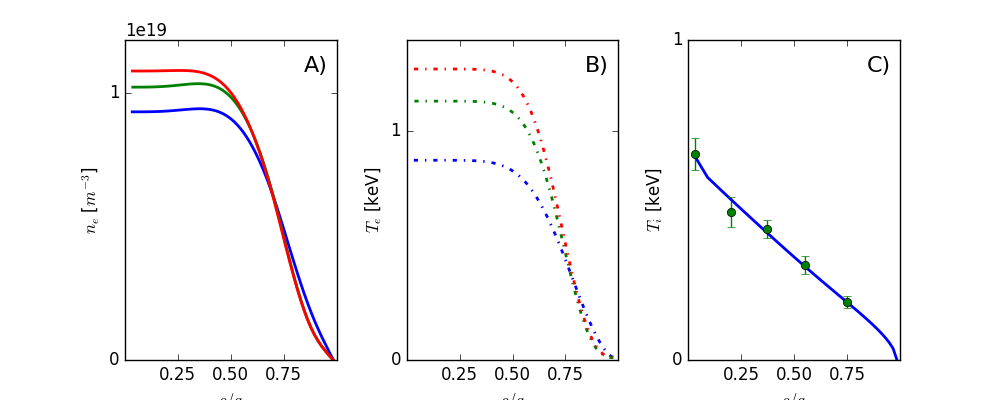
\includegraphics[width = 1.\linewidth]{./plots/model_inputs}
	\label{fig:model_inputs}
	\caption{Key input parameters to the model. A) is the electron density provided by FIR, B) is the electron temperature provided by TS, and C) is the ion temperature at 12ms from CHERS measurement used for initial condition.}
\end{figure}%

The forward model predicts the evolution of the
1-D $T_i$ profile by incorporating input signals from a range of plasma
diagnostics to calculate the classical heat balance terms. These diagnostics include Thompson Scattering(TS) measurements of $T_e$\cite{Kubala2016UpgradesDiagnostic, DenHartog2010Pulse-burstScattering}, the Far-InfraRed Interferometer and Polarimeter(FIR) measurements of $n_e$ and
Faraday rotation\cite{Yates2008SimultaneousMST, Brower2001MultichannelPinch}, and $D_{\alpha}$ emission measurements. Additionally, the model also includes equilibrium reconstruction via MSTFIT\cite{Anderson2004EquilibriumPinch}, as well as neutral modeling through
DEGAS2\cite{Stotler1994Neutral2,Stotler1994Neutral2}. The impurity density is assumed to be constant in the period of
interest based on previous measurements \cite{Kumar2012a,Nornberg2018IncorporatingCharge}. The
model further uses an initial temperature profile from measurements via Charge Exchange Recombination Spectroscopy\cite{DenHartog2006Advancesinvited}, as initial ion temperature profile is governed by reconnection heating and stochastic transport during start-up conditions. 

\section{Neutral Dynamics and Charge exchange}\label{sec:neutral}

Charge exchange collisions cause neutral atoms to donate an electron to thermal ions thereby creating a hot neutral and a cold ion, representing a heat loss for the ions. In PPCD plasmas where other
loss mechanism are reduced, charge exchange loss becomes dominant. 

In previous estimates, the neutral fluid is assumed to be cold, therefore, if a
thermal ion undergoes charge exchange it represents a total energy loss. This
assumptions is incorrect. The mean free path of a room temperature neutral is
very short (<1cm), even in a typical edge plasma, where as thermal neutrals created
via charge exchange have a much longer mean free path. Consequently, neutrals
penetrating to the core are mostly generated near the mid-radius and therefore
have a temperature comparable to mid-radius ions. At the same time,
calculations conclude that a charge exchange neutral created in the core of
the plasma, if traveling through core-like conditions, has a mean free path
shorter than the minor radius, implying a fraction of such neutrals would
undergo secondary ionization or charge exchange reactions.  At the same time,
with a long mean free path compared to the minor radius ($Kn \simeq 0.8$), the
neutral species cannot be adequately treated as a fluid. 

$D_{\alpha}$ emission is dominated by emission in
the plasma edge where neutral density is high. As the core contributes
negligible emissions, a simple inversion of line integrated measurements has
difficulty capturing anything more detailed than an upper bound of the core neutral density.
Therefore, physics-based equilibrium modeling is needed to construct self-consistent core neutral profiles that produce the observed $D_{\alpha}$ emissions. There was a previous attempt to incorporate a simpler Monte Carlo simulation to determine neutral density, but it needed a spatially uniform anomalous neutral particle source at 50eV, and still performed poorly when fitting PPCD data. Additionally, previous work using neutral density as part of impurity charge state balance calculations found that the core neutral density was likely over predicted.[[TODO:Cite Tulio and Santhosh papers.]

\begin{figure}
	\centering
	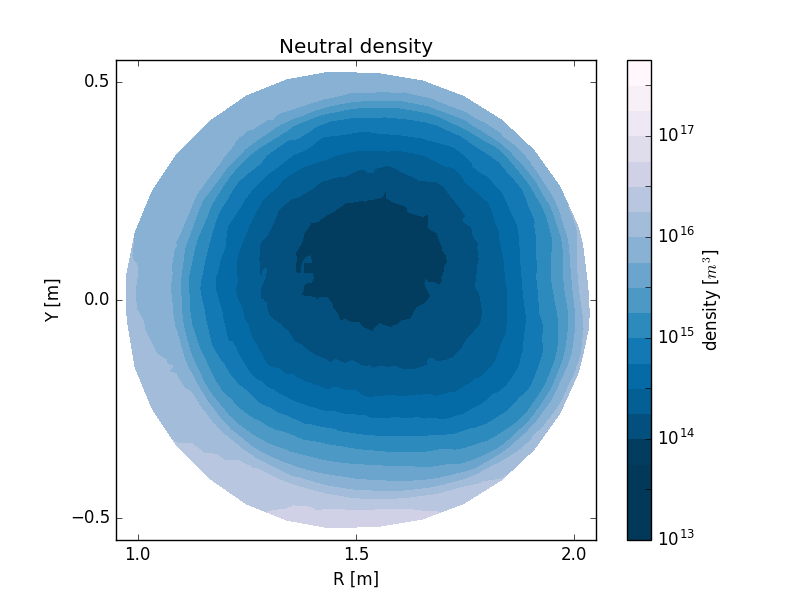
\includegraphics[width = 1.\linewidth]{./plots/degas_neutral_n}
	\caption{Typical neutral density result from DEGAS2 show a rapid drop off towards the core. There are two notable asymmetries: the Shafranov shift result in lower neutral density on the outboard side, and the gas puffing prior to the PPCD period leaves a residual up/down asymmetry.}\label{fig:DEGAS2_2d_density}
\end{figure}%

For this work, DEGAS2, a 2-D Monte Carlo simulation that produces neutral density and
temperature profiles\cite{StotlerDEGAS2Manual}, is incorporated to model core neutral profiles. DEGAS2
use  $ T_{e} $ and $ n_{e} $ profiles as input, and it tracks and tallies
charge exchange, ionization, recombination, and molecular disassociation
reactions, as well as associated particle and heat flow of test particles.
Synthetic $ D_{\alpha} $ radiance measurements are created within DEGAS2, and they are
used to fit experimental measurements by varying boundary source rates
as fitting parameters. The precise mechanism behind this neutral source, such
as recycling, is outside of the scope of this work. A three surface source
geometry, each having an independent source rate is used, consisting of an
outboard limiter, a pumping duct region (bottom 45\textdegree) and the rest of
the wall. The outboard limiter is singled out for special attention due to the
Shafranov shift causing the last closed flux surface to strike the outboard
limiter rather than the inboard. Treating the pumping duct as a separate source is necessary to improve the fit quality in PPCD conditions. The sources
and their contributions to the plasma are assumed to be linearly independent as
neutral-neutral interaction is negligible. An example of the result of the
DEGAS simulation for a single shot and time is shown as Fig~\ref{fig:DEGAS2_2d_density} and~\ref{fig:temp}.

\begin{figure}
	\centering
	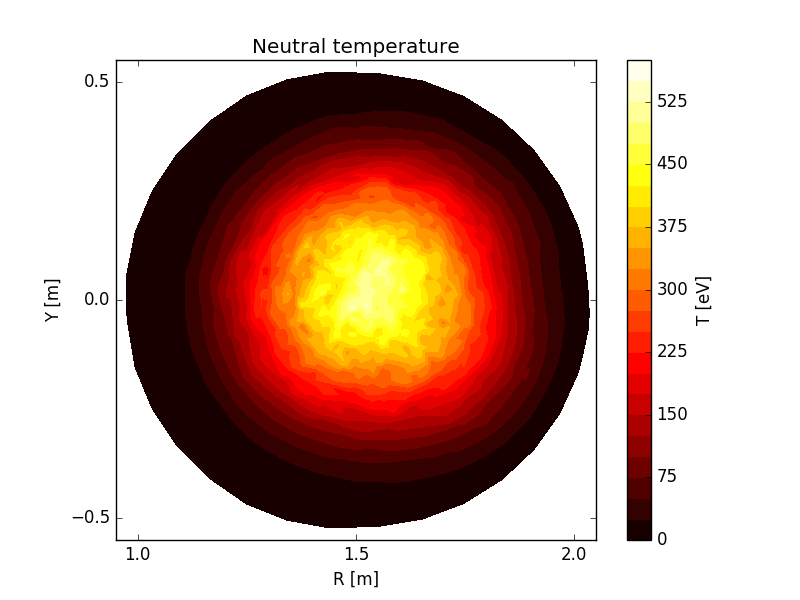
\includegraphics[width = 1.\linewidth]{./plots/degas_neutral_t}
	\caption{Neutral modeling results also show a corresponding `rise' in temperature as one moves towards the core. This produces a charge exchange loss profile that is both lower and more hollow than estimates assuming cold neutrals.}\label{fig:temp}
\end{figure}

DEGAS2 simulations are evaluated at 0.5ms intervals due to both the
computational cost of the Monte Carlo simulations, and the frequency at which $
T_e $ measurements, a key input, are available via TS. The 2-D results are
incorporated into the 1-D ion thermal model through flux surface averaging.

DEGAS2 modeling shows $\frac{T_{neutral}}{T_{i}} \simeq 0.7$ in the core, which combined with lower $ n_{neutral} $ leads to
lower charge exchange heat loss than previous estimates. Further, the charge
exchange loss is found have a hollow profile (see Fig. \ref{fig:dedt_plot}), and is at a level that is broadly
consistent with the temperature evolution of the ions without having to invoke
additional anomalous heating terms during PPCD periods. 

\section{Flow related effects on heat}\label{sec:flow}

In previous power balance work, the heat lost to particle flow (often called $P_{conv}$) is one of the largest terms\cite{Fiksel2006}. Calculating $P_{flow}$ involves estimating the ion
particle flux.  However, no diagnostic measurements of $n_i$ in MST is
available, therefore, $n_i$ is inferred indirectly through the evolution of
$n_e$ combined with previous work on characterizing the impurity content in
PPCD\cite{Kumar2012,Nornberg2018IncorporatingCharge}.

MSTfit uses the 11-chord line integrated $n_e$ measurement from the FIR
interferometer to reconstruct the density profile. Measurements show a clear rise of
core electron density in the early half of the PPCD period, ending around 16.5ms. It is
important to determine the nature of this density rise, as the temperature of
these ``new" ions would have a significant effect on the model predictions.

The DEGAS2 simulations characterizing the neutral dynamics also provide a
tally of the electron source rate due to the ionization of the neutrals. This
source primarily concentrates in the edge and is too low in the core to account
for the density rise in the core (Fig. \ref{fig:ne_change}). The further
ionization of impurities due to increasing temperature is another possible
source. Impurity contribution to the electron density rise is estimated using
previous measurements, including carbon, aluminum, oxygen and boron\cite{Kumar2012a, Nornberg2018IncorporatingCharge}. Their contribution to the electron source
rate is calculated from the change of charge state balance and is also found to be negligible.


\begin{figure}
	\centering
	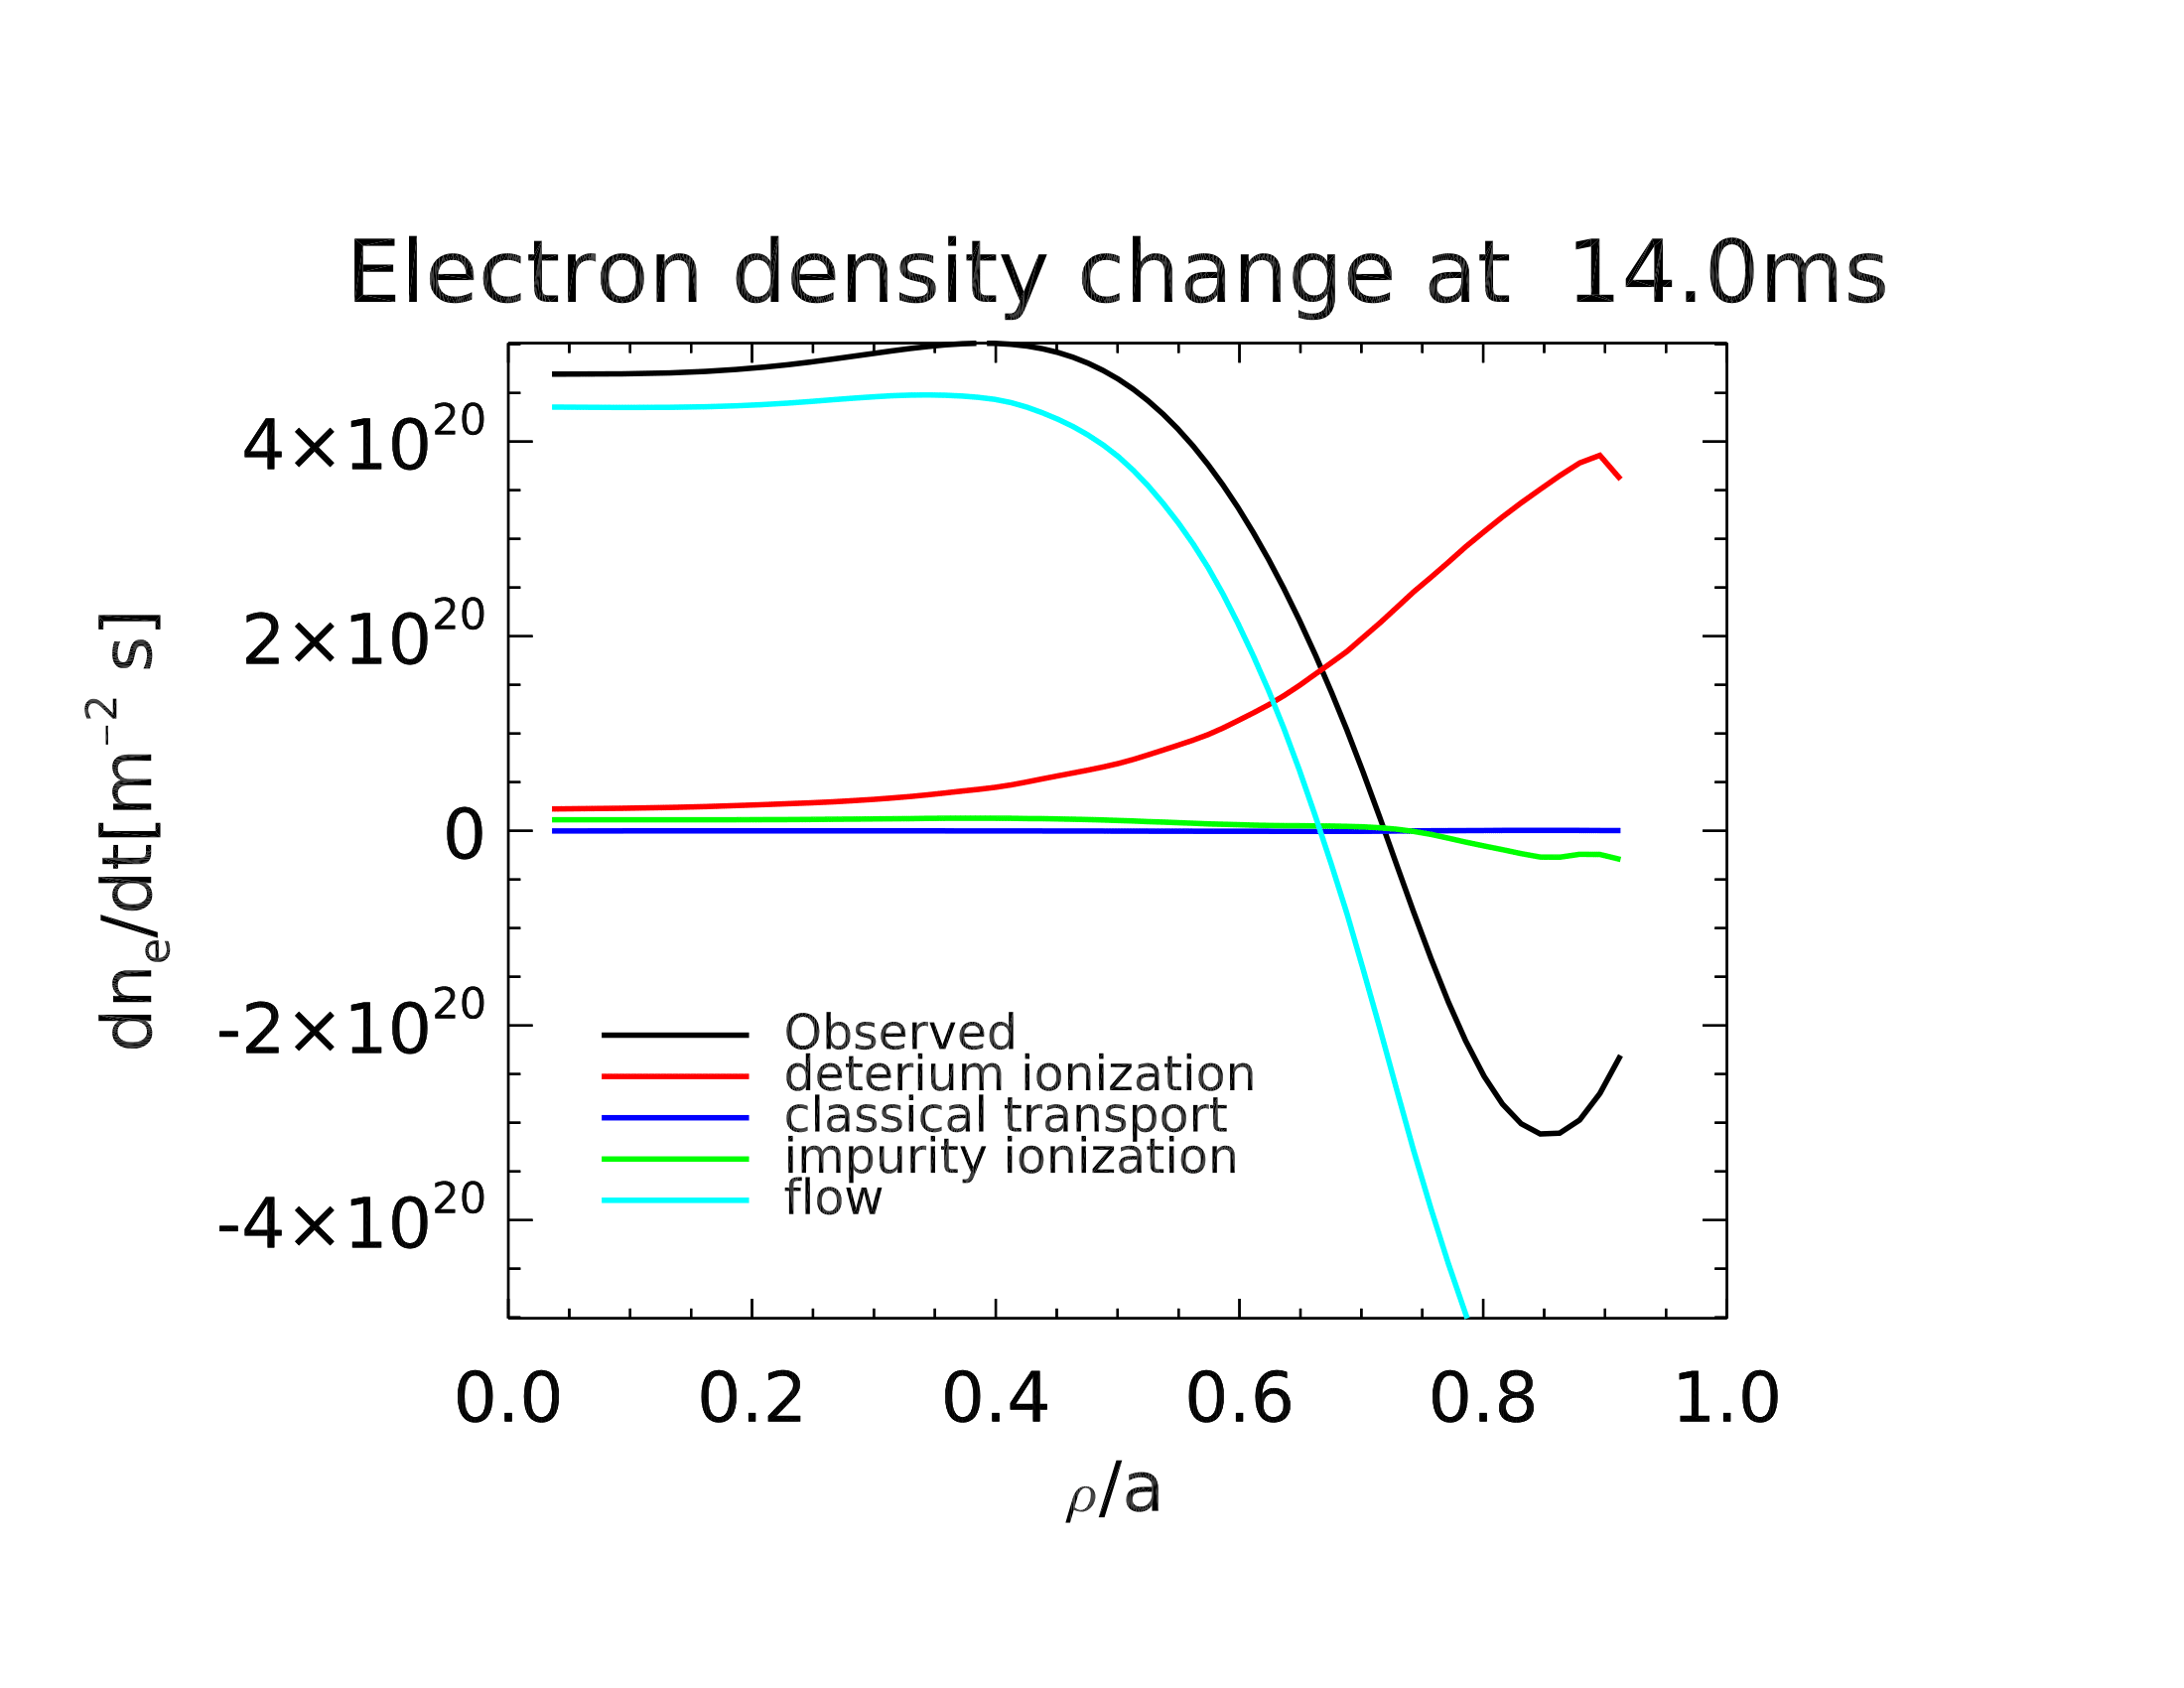
\includegraphics[width=0.95\linewidth]{./plots/dndt_at14-1}	
	\caption{Profiles of electron density change show that the $n_e$ source terms are concentrated at the edge, and thus the core density rise needs to be accounted for by flux.}
	\label{fig:ne_change}
\end{figure}

\begin{figure}
	\centering
	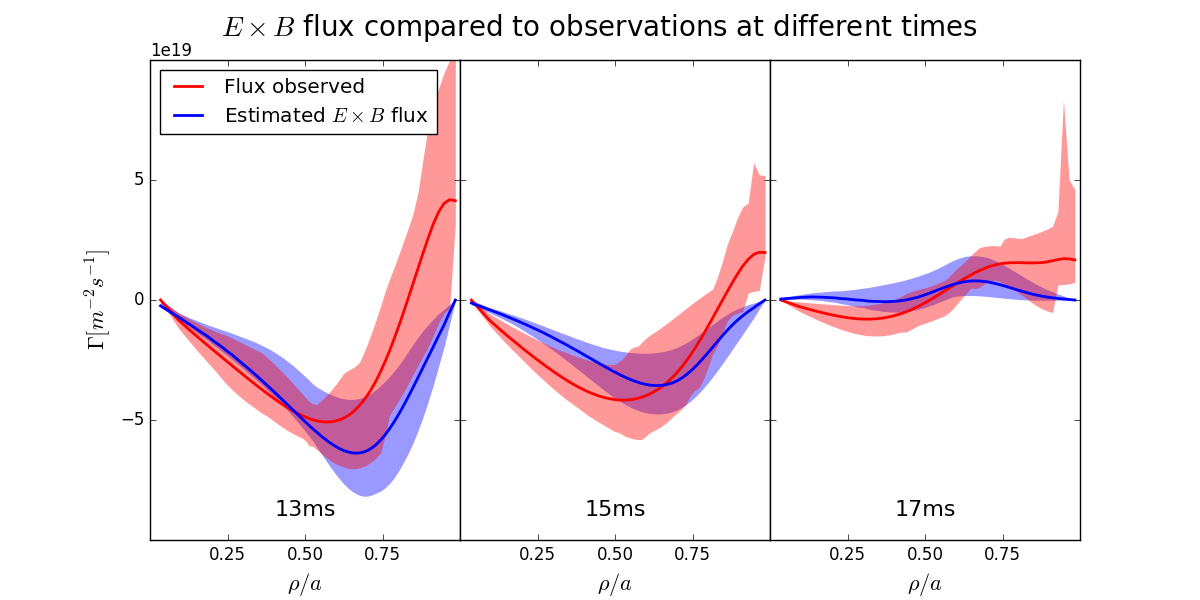
\includegraphics[width=0.95\linewidth]{./plots/flux_comp}
	\caption{Estimated flux values. The calculated $ E\times B $ flux is in red. It goes to zero at the edge as the density goes to zero.}
	\label{fig:flux_compare}


\end{figure}

The calculated electron source rates are insufficient to account for the
density rise, and thus there must be an inward particle flux. The particle flux
($\Gamma_{obs}$) needed to satisfy the continuity equation (\ref{eqn:cont}) is
then calculated. However, we seek to confirm the theoretical plausibility of an
inward pinch by considering the evolution of the magnetic equilibrium.

Although radial E fields has been measured in the past using Heavy Ion Beam Probe, and well as capacitive probes, it does not constrain the
radial $\Gamma_{\vec{E} \times \vec{B}}$. Instead, the slow time-scale E field
is estimated using the evolution of reconstructed B field from edge flux coil
and FIR polarimetry data. The radial flux, $\Gamma_{\rho} = n_e\frac{(\Vec{E}\times\Vec{B})_{\rho}}{B^2}$, is constrained by $E_{pol}$ and $E_{tor}$. The MSTfit equilibrium reconstruction outputs
reconstructed flux values and flux surfaces in 2D which enables the calculation of $E_{pol}$ and $E_{tor}$. In particular $E_{pol}$ can be calculated through:

\begin{align}
E_{pol}(\rho_v) & = \int_{0}^{\rho_v}\rho_v' \frac{dB_{tor}}{dt} d\rho_v'
\end{align}

where it is taken as a boundary condition that the $E_{pol}$ is zero at
the magnetic axis.

%where $\rho_v$ is the flux surface averaged minor radius.

Calculating $E_{tor}$ is slightly more complicated, as it is a function of major
radius and not $\rho$. On MST, there is a poloidal gap (circles around the vessel poloidally) in the conducting wall and the voltage measured across the gap ($V_{PG}$) is a reflection of the toriodal E field at the wall. To incorporate into the 1-D approximation, $E_{tor}(R, Z=0)$ along the
Z = 0 plane is determined as a function of major radius (R) through equation
(\ref{eqn:E_tor}) and the boundary condition implied by $V_{PG}$. The results and
then averaged according to flux surface. 

\begin{align}
E_{tor}(R) & = -\frac{1}{\int_{R_0 - a}^{R_0 + a} R' \frac{\partial B_{pol}}{\partial t} dR'} - E_{tor}^{boundary} \label{eqn:E_tor}\\
E_{tor}^{boundary} & = \frac{- V_{PG} }{2 \pi R_0}\label{eqn:E_tor_bc}
\end{align}
where $R$ refers to the major radius.

Since the $ \frac{dB}{dt} $ term cannot be evaluated directly, sequential
MSTfit reconstructions, 0.5ms apart are used to provide $ B_{pol} $ and $
B_{tor} $ information from which a numerical derivative is calculated. The results show $E_{tor}$ to
be relatively stable in the core, but changes direction in the edge as time
progresses. This reversal correlates with current drive being exhausted in the
edge. Note this is not related to the edge $\vec{B}$ reversal that gives RFP it's name.

From there the radial particle flux is calculated as:

\begin{equation}
\Gamma_{\vec{E} \times \vec{B}} = n_{e} \frac{E_{pol}B_{tor} - E_{tor}B_{pol}}{B^2}
\end{equation}

This is compared to $\Gamma_{obs}$ previously calculated from Eqn. \ref{eqn:cont} and shown in figure \ref{fig:flux_compare}. For the core to about the
mid radius, the estimated $\Gamma_{\vec{E} \times \vec{B}}$ tracks the flux
needed to account for density change well. However, further into the edge, there
is residual flow outwards since the neutral ionization rates are faster than
density growth, thus particle loss is need to balance the continuity equation.
This is likely caused by transport mechanisms such as turbulence due to
drift wave activity\cite{Duff2018ObservationPlasmas,Williams2017TurbulencePinch,NishizawaPRLSubmitted}.

Importantly, the $ E_{tor} $ reversal during the PPCD period causes the
estimated $ \Gamma_{\vec{E} \times \vec{B}} $ flow to cease. This echoes MHD
calculations by J. Reynolds that found the $ E \times B $ flow would cease as
the axial E field is reduced and reversed\cite{ReynoldsThesis}.

\begin{figure}
	\centering
	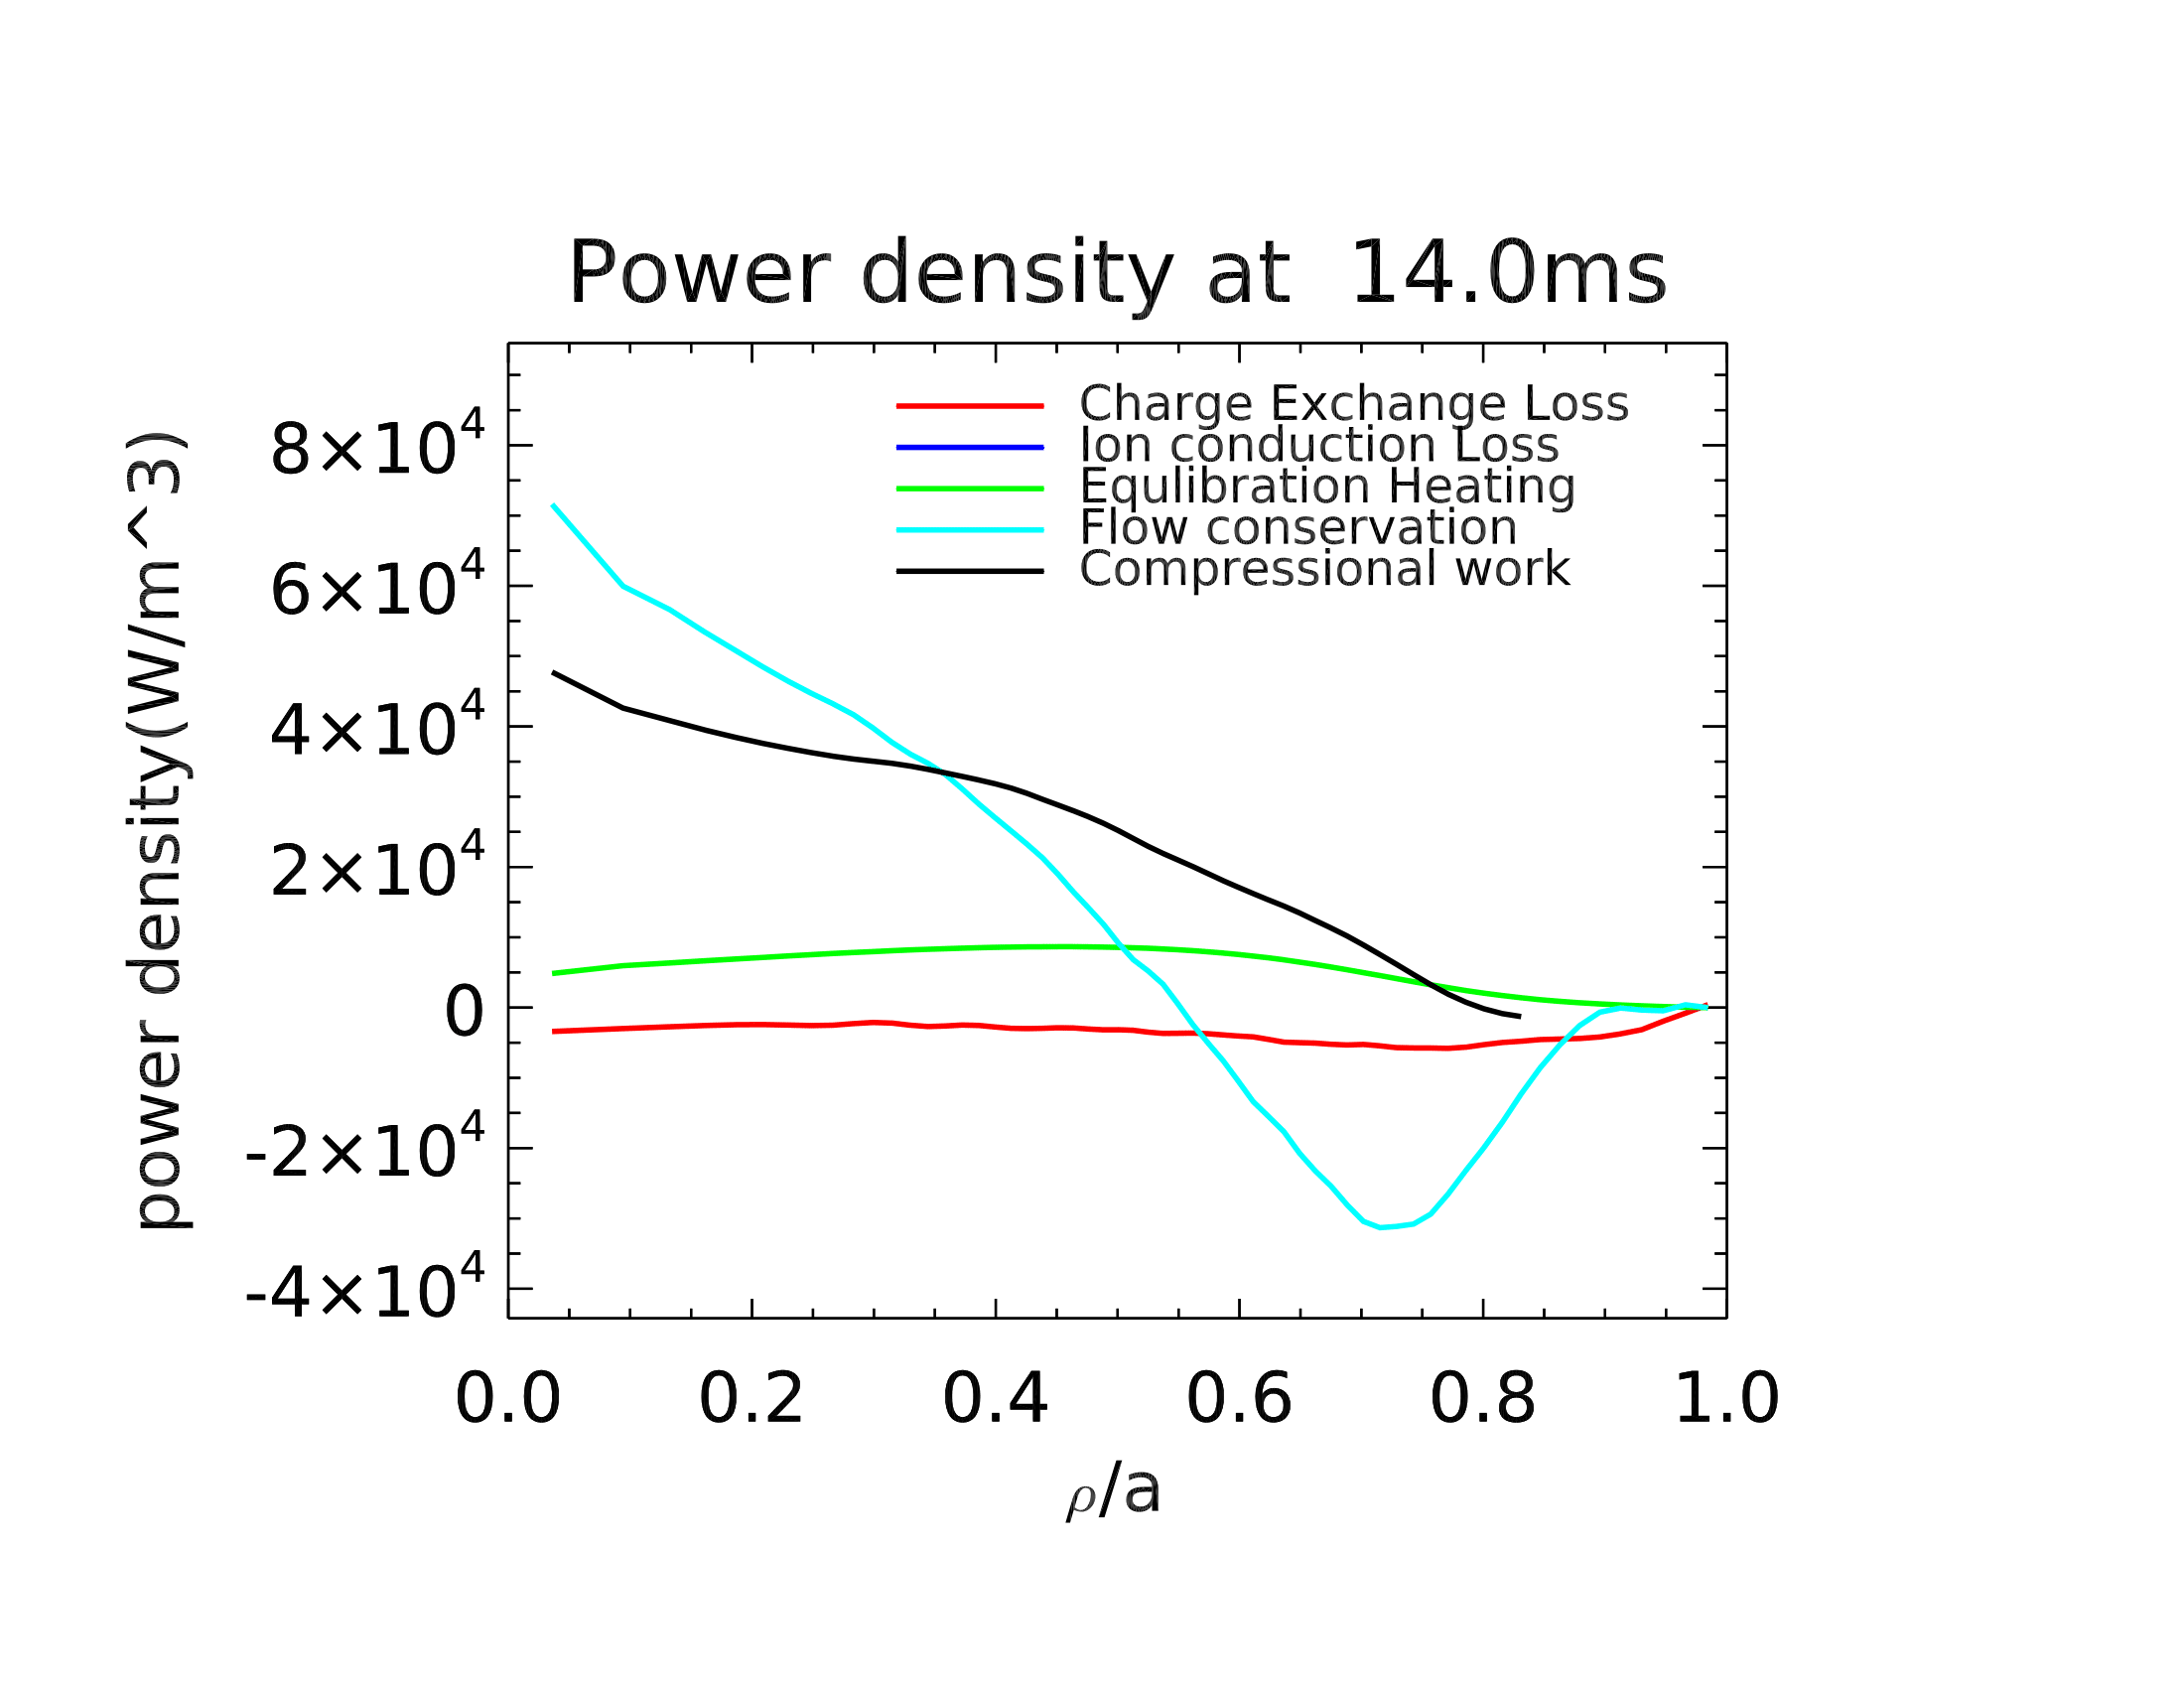
\includegraphics[width=1.\columnwidth]{./plots/dedt_june18-1.png}
	\caption{Flow effects are the most significant contributors to the forward model, although the conservation term (in light blue) is essentially moving thermal energy from outer-mid radius regions to the core. In the absence of the radial flow induced terms, the equlibration and charge exchange terms are relatively equal. \label{fig:dedt_plot}}
\end{figure}

Using $\Gamma_{obs}$, the flow
contribution to heat balance is calculated using Eqn. \ref{eqn:flux_terms} and found to be the largest term in
the core of the plasma (Fig. \ref{fig:dedt_plot}). Breaking it down further, the notable observation is
that the compression heating is larger than the equlibration heating and is the
largest heating term in the core. The conservation term is larger, but does not
cause temperature rise as it represents the thermal energy carried by the particle inflow. The temperature in the core is predicted to rise slightly
while in the gradient region it would decrease as the colder ions flow in.

\section{Prediction and measurement of ion temperature}


To assess the applicability of the model, it's predictions are compared to
measurements of $T_{C^{6+}}$ using Charge Exchange Recombination
Spectroscopy\cite{DenHartog1994,DenHartog2006Advancesinvited}. CHERS
measurements of C+6 temperature are used as a proxy for majority ion temperature
for model comparisons. Since $\tau_{C^{+6}-D^{+}} \approx 0.5ms$ is small compared to the time
scale of analysis, it is taken as a proxy of majority ion temperature because direct
measurement is not available\cite{Reardon2003}. The primary drive that brings
the two temperatures out of equilibrium are sawtooth events which are
suppressed in PPCD plasmas\cite{Fiksel2009}. Since MST's CHERS system can only
measure temperature at one location at a time, the profile is constructed from
an ensemble of measurements at different locations fitted to a two power
profile across the radius.

\begin{figure}[!ht]
	\centering
	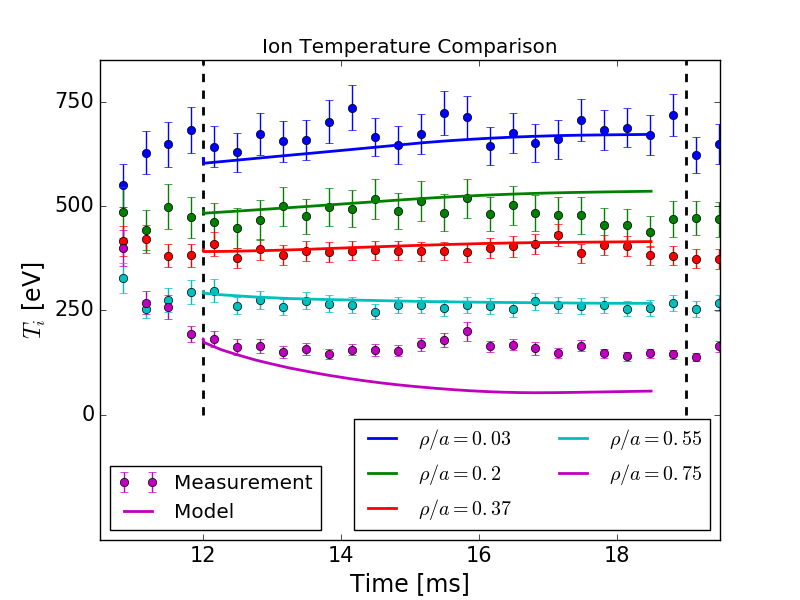
\includegraphics[width=0.95\columnwidth]{./plots/temp_comp_ext_full}
	\caption{Temperature prediction vs observations. The classical thermal transport model is able to successfully prediction $T_i$ evolution during PPCD up to $\rho /a = 0.55$. Note that model does not initialize at exactly the observed value at a given chord as it is fit to a smooth profile in the radial direction.\label{fig:comp}}
\end{figure}

The model is initialized with $T_i$ profile obtained by fitting CHERS
measurement at 12ms. The time is chosen for being the earliest time that PPCD
consistently suppresses tearing mode activity. The model is then allowed to
propagate until 19ms, and its prediction of $T_i$ is compared to the
temperature measurement from an ensemble of plasma shots where PPCD was
successful. The result of this comparison is show in fig. \ref{fig:comp}.
Notably, the model was able to predict the maintenance and slight rise in
temperature without invoking any anomalous heating. The model, however,
performed poorly in the $\rho /a \approx 0.75$ region, indicating that there are might be residual anomalous heating in the edge region associated with tearing mode fluctuations. This discrepancy echos the same in the particle transport discussed in section \ref{sec:flow} in its location, but not in it's nature. 

\section{Discussion}
Previous estimations that resulted in the $T_i$ being considered anomalously
high suffered from the inadequate estimation of the neutral
interactions\cite{Fiksel2006,BiewerThesis, Wyman2007}. The calculation used was based on
simple inversions of the $D_{\alpha}$ emission, and it impacted the ion transport
calculations in two ways. First, the calculation of the CX loss term, where the
overly high estimate of core $n_n$, as well as the assumption of total loss
(ie. cold neutrals) resulted in the overestimation of CX loss. The warm neutrals represent a transport-like process as their energy comes from the fact that they are the product of prior charge exchange reactions. Secondly, the
overestimation of the source term led to overly high estimates of
outward particle flux, therefore overly high convective losses. The proper
accounting of the neutral dynamics is crucial to the proper
accounting of ion thermal transport. 

A further area of improvement upon the previous estimations is the treatment of $\frac{\partial}{\partial t}$ terms. In the works cited above, ion thermal transport was approached as heat balance in quasi-equilibrium, where the time derivatives are assumed to be not significant. However, due to the transient nature of inductively driven PPCD \cite{Sarff1995TransportPinch}, the equilibrium is steadily evolving, and  the time derivatives are important as the density and temperature profiles are evolving at similar time scales over the time period of interest. This impacts the model most directly in the calculation of particle flux.

%Recent development in the Tokamak world also moving towards more detailed evaluation of the neutrals' impact on transport calculations by coupling neoclassical PIC code to Monte Carlo neutral transport code\cite{Stotler2013PedestalCode}.

%At the same time, neutral density have long been suspected to affect the L to H transition in Tokamaks, and there have been renewed interest in the modeling neutrals in plasma experiments such as on DIII-D\cite{Stotler2013PedestalCode}, NSTX\cite{Stotler2015MidplaneExperiment} and measurement in HIT SI\cite{Elliott2016Two-photonNeutrals}. Despite the neutral profiles impacting the ion transport characteristics directly through both the charge exchange loss term, as well as indirectly through it's impact on ion source geometry and therefore the particle balance and particle flux, detailed accounting of the neutrals have not been performed on MST prior to this work.

The possibility remains for anomalous heating localized around the edge/reversal surface region. Though it is relevant to note that as a foreword model, discrepancies are cumulative. Further, the lower than observed temperature in the edge region of the model did not impact the transport prediction in the core region. The region of discrepancy corresponds with the region calculated to lose power to the $\frac{3}{2}\vec{\nabla}\cdot(p\vec{V})$ term, corresponding to the existing ions flowing inwards and being replaced with colder ions. Hence this discrepancy may also be indicative of higher than modeled ion temperature further out in the plasma, either through stochastic heating from drift wave turbulence\cite{Fiksel2009}, or due to the fact that the model assumed all wall recycling particles are cold. 

This model ignores neoclassical transport since it is expected
to be small for ions in the RFP. Despite the fact that deuterium is expected to be in the
banana regime in MST\cite{Kumar2012a}, the neoclassical transport is expected to be smaller
than classical as $\frac{q^2}{\epsilon^{3/2}} \leq 0.2$ everywhere in MST, where $\epsilon$ is the inverse aspect ratio.
More significantly, turbulent transport is also ignored, and
this likely causes the inability for the classical model to predict $T_i$
evolution at $\rho /a \approx 0.75$ as discussed above.  While the ion transport at the edge is likely limited by turbulence, inside of $\rho/a = 0.55$ however, turbulence does not seems to play a significantly role. Unlike the electron temperature, the ion temperature not only maintains it's core peaking, it becomes more peaked due to the inward particle flux.

%Read the OFCD papers again. It may echo the observations regarding compressional heating.
Finally, the successful modeling of tearing suppressed RFP plasma provides a baseline to investigate deviations from the successful tearing reduction. For example, PPCD occasionally experience a burst of magnetic activity associate with the m=0 mode then rapidly returning to well confined PPCD conditions much faster than a sawtooth event. The associated reconnection heating could be studied with more clarity than heating associated with the more violent and chaotic sawtooth events. 

\section*{Acknowledgement}
The author would like to thank the assistance of Dr. J. Anderson,  Prof. Darren Craig, and Dr. J. Duff. This work is supported by the U.S. Department of Energy, Office of Science, and
Office of Fusion Energy Sciences under Award Number DE-FC02-05ER54814.


% If in two-column mode, this environment will change to single-column format so that long equations can be displayed. 
% Use only when necessary.
%\begin{widetext}
%$$\mbox{put long equation here}$$
%\end{widetext}

% Figures should be put into the text as floats. 
% Use the graphics or graphicx packages (distributed with LaTeX2e).
% See the LaTeX Graphics Companion by Michel Goosens, Sebastian Rahtz, and Frank Mittelbach for examples. 
%
% Here is an example of the general form of a figure:
% Fill in the caption in the braces of the \caption{} command. 
% Put the label that you will use with \ref{} command in the braces of the \label{} command.
%
% \begin{figure}
% \includegraphics{}%
% \caption{\label{}}%
% \end{figure}

% Tables may be be put in the text as floats.
% Here is an example of the general form of a table:
% Fill in the caption in the braces of the \caption{} command. Put the label
% that you will use with \ref{} command in the braces of the \label{} command.
% Insert the column specifiers (l, r, c, d, etc.) in the empty braces of the
% \begin{tabular}{} command.
%
% \begin{table}
% \caption{\label{} }
% \begin{tabular}{}
% \end{tabular}
% \end{table}

% If you have acknowledgments, this puts in the proper section head.
%\begin{acknowledgments}
% Put your acknowledgments here.
%\end{acknowledgments}

% Create the reference section using BibTeX:

%\printbibliography
\bibliography{mendeley_v2,thesis,supplement}
%\bibliography{mst_xing.bib,mendeley_v2.bib}
\bibliographystyle{apsrev}
\end{document}
%
% ****** End of file aiptemplate.tex ******
